\chapter{Background from Beam Dumps}
\label{BeamDumps}
After the collision of the \positron\electron beams, the spent beams are directed through the extraction line (EXT) of the ILC towards the beam dumps. The beam dumps basically consist of tanks, filled with water at a pressure of \SI{10}{\bar} and surrounded by iron and concrete shieldings. The choice of a water tank as the beam dump is based on the high specific heat capacity of water, which is ideal to dissipate the energy of the beams. Therefore the water beam dumps for the ILC are designed to absorb the beam power of \SI{17}{\mega\watt} at \SI{500}{\GeV} centre of mass energy.\\
Dumping a high energy lepton beam in a water tank means on the other hand the emission of neutrons of high and low energies. Not only the effect of these neutrons reaching back to the detectors at the interaction point, but also the doses that the surrounding area would suffer from, are the centre of interest in this chapter. The higher occupancy in the detectors is a small effect of the neutrons, whereas the damage of the detector components and the irradiation of the surrounding are the more severe consequences. Neutron background would on the one hand lead to displacement damage in the silicon sensors, which results in charge traps, reduction of charge transfer and the overall degrading of the detector performance. On the other hand, the irradiation of the surrounding leads to restricted access of the accelerator tunnel and activates all present components.\\It is therefore crucial to understand the level of neutron background generated by every beam bump of the ILC beam trains.

\section{\fluka and \flair}
\label{BeamDumps:fluka}
\fluka is known to be a very accurate Monte Carlo simulation tool in respect of simulating low energy neutrons. After providing the simulation settings and the geometry in a text file as input source, \fluka uses certain algorithms to simulate and track the particles through the geometry.
%TODO: FLUKA algorithms
The graphical interface developed for \fluka is called \flair. Its plug-in flair-geoviewer allows interactive geometry viewing and editing, as well as debugging and three dimensional visualization.

\section{Beam dump design}
\label{BeamDumps:design}
The design for the beam dump simulated for this thesis is based on the TDR design as well as on the technical design drawings done by B. Smith~\cite{Smith_drawings}.
Figure~\ref{fig:BeamDumps:geometry} shows the visualization of the beam dumps modelled within \fluka. It is a simplified version derived from the design drawings, only containing a simple water tank in the middle of the shielding in the beam dump tomb. The infrastructure, like cables, water pipes etc., is not included in the simulation geometry.

\begin{figure}
\begin{center}
\resizebox{.9\textwidth}{!}{%
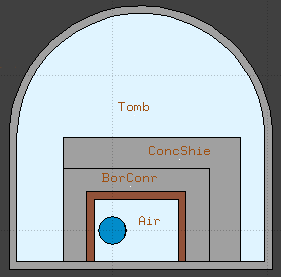
\includegraphics[height=0.35\textheight]{Front_view_BeamDump_Tomb.png}%
\quad
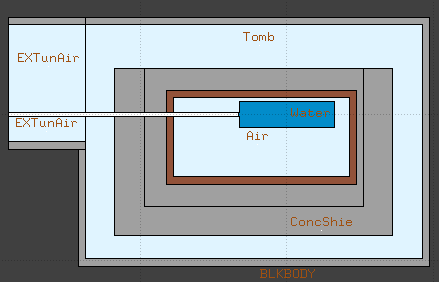
\includegraphics[height=0.35\textheight]{Bird_view_BeamDump_Tomb.png}%
}
\caption[Geometry of the simulated beam dumps.]{The beam dumps modelled within \fluka and visualized with \flair. On the left hand side, the front view on the beam dump is shown, i.e. the beam direction is going into the paper plane, whereas the right hand side shows the top view. The actual dump is represented by the water tank in the middle of the different shielding walls. A \fluka specific feature is the need of having a black body void around the geometry. This void is the limit of the tracking region and stops all particles reaching this edge.}
\label{fig:BeamDumps:geometry}
\end{center}
\end{figure}


\section{EXT line lattice}
\label{BeamDumps:lattice}
\section{Simulation studies of neutrons reaching the IR}
\label{BeamDumps:simulation}
